\subsection{Testing approximate scaling beyond one-lag magnitudes}
\label{sec:transport-temporal-scaling}

The visible collapse motivates a stronger, independently evaluated claim:
does one scalar exponent approximately preserve signed displacement laws and
their dependence across two consecutive intervals? The answer is substantially
more favourable on \SIrange{100}{1600}{\second} than across the full range.
This is evidence for approximate scaling at a stated temporal and distributional
resolution, rather than exact self-similarity of the whole process.

\paragraph{A temporal observable and common observations.}
Write $\mathbf X_1=\mathbf r(t+\tau)-\mathbf r(t)$ and
$\mathbf X_2=\mathbf r(t+2\tau)-\mathbf r(t+\tau)$. The measured vector is
\begin{equation}
 \mathbf Z_\tau=(X_{1,E},X_{1,N},X_{2,E},X_{2,N}),\qquad
 \widetilde{\mathbf Z}_\tau=
 \frac{\mathbf Z_\tau}{s_0(\tau/\tau_0)^{H_*}}.
 \label{eq:two-interval-scaling}
\end{equation}
The invertible transformation $(\mathbf X_1,\mathbf X_2)\mapsto
(\mathbf X_1,\mathbf X_1+\mathbf X_2)$ connects this observable to positions
relative to the same origin at times $\tau$ and $2\tau$. For an $H$-self-similar
process with stationary increments, its law must be invariant under this common
rescaling. Here the origins are pooled within observed flights; stationarity of
those increments is not established by this comparison.

Three lag grids, in seconds, were fixed before running this extension:
\[
 \begin{aligned}
  \text{full:}\quad &(10,100,1000,10000),\\
  \text{intermediate:}\quad &(100,200,400,800,1600),\\
  \text{long:}\quad &(1000,2000,4000,8000).
 \end{aligned}
\]
They probe the full, intermediate and long intervals suggested by the preceding descriptive analysis;
their boundaries are not inferred crossover times. Within each grid, every
10-s origin with uninterrupted support through $2\tau_{\max}$ is retained in
every eligible segment. The same flights and origins enter every lag. Cleaning
boundaries are never crossed. Origins receive equal weight within a flight,
and flights receive equal total weight. The required support is therefore
20000, 3200 and 16000 seconds, respectively. Different grids admit different
populations; their comparison does not isolate a lag effect from flight selection.

\paragraph{Separate fitting and evaluation.}
A fixed hash of the calendar date assigns approximately half the dates to
training and half to validation, with the same assignment in both disciplines.
All eligible flights with valid dates enter one of these roles. Three
intermediate-range paraglider flights have invalid catalogue dates and are
excluded; no other eligible flight is excluded for this reason.
On training flights only, the inverse-CDF quantiles of $|X_{1,E}|$, $|X_{1,N}|$
and $|\mathbf X_1|$ at probabilities $.25,.50,.75,.90$ are fitted against lag
in logarithmic coordinates. $H_*$ is the unweighted mean of the twelve slopes.
The reference time $\tau_0$ is the smallest lag of the grid, and $s_0$ is its
training radial median. Both are then held fixed on validation flights.
There is no lag-specific centring, rotation, whitening or marginal adjustment.
For bounded memory, training quantiles use 8192 logarithmic bins between
$10^{-6}$ and $10^7$ metres, with separate underflow and overflow counts.
Geometric bin centres bound the quantile discretisation error by 0.183\%;
the corresponding deterministic slope-error bound is recorded for each grid.
This approximation concerns training only: validation probabilities are counted
directly from the signed increments.

\begin{table}[tb]
 \centering\small
 \caption{Training and validation populations for the two-interval comparison.
 Days and origins refer to validation; the training quantile fit supplies $H_*$.}
 \label{tab:temporal-scaling-population}
 \begin{tabular}{llrrrrr}
\toprule
 & Lag range (s) & Train & Validate & Days & $H$ & $n_{\rm orig,val}$\\
\midrule
Para & 10--10000 & 7149 & 7211 & 902 & 0.899 & 3598452\\
Para & 100--1600 & 74267 & 75561 & 2997 & 0.915 & 59782745\\
Para & 1000--8000 & 13252 & 13725 & 1339 & 0.905 & 7680809\\
Hang & 10--10000 & 281 & 282 & 198 & 0.884 & 119993\\
Hang & 100--1600 & 2934 & 2980 & 938 & 0.899 & 2639959\\
Hang & 1000--8000 & 609 & 631 & 348 & 0.914 & 294973\\
\bottomrule
\end{tabular}

\end{table}

\paragraph{What agreement is tested.}
The four coordinate projections and all twelve unit-normalised pairwise sums
and differences define a fixed set $\mathcal U$ of 16 directions in
$\mathbb R^4$. In particular, $(X_{1,E}-X_{2,E})/\sqrt2$ compares consecutive
eastward displacements and is sensitive to changes hidden by their separate
marginals. CDFs are evaluated at the fixed dimensionless thresholds
$\mathcal A=\{0,\pm0.1,\pm0.25,\pm0.5,\pm1,\pm2,\pm4,\pm8\}$.
For validation flights $f=1,\ldots,F$, with $n_f$ common origins, define
\begin{equation}
 \widehat F_{\tau,u}(z)=\frac1F\sum_f\frac1{n_f}
  \sum_i\mathbf1\{u^\mathsf T\widetilde{\mathbf Z}_{fi,\tau}\le z\},
 \qquad
 \widehat D_{\mathcal U'}=
 \max_{\tau<\tau',\,u\in\mathcal U',\,z\in\mathcal A}
 |\widehat F_{\tau,u}(z)-\widehat F_{\tau',u}(z)|.
 \label{eq:temporal-projection-distance}
\end{equation}
The spatial set uses $E_1,N_1,(E_1+N_1)/\sqrt2,(E_1-N_1)/\sqrt2$;
the temporal set contains the remaining twelve directions, involving the second
interval. All projections would characterise a joint law, but this finite set
does not~\cite{fraiman2022}. It measures agreement at specified directions and
thresholds, including signs and some temporal dependence, rather than a bound on
the full four-dimensional distribution or its tails.

For uncertainty, 999 bootstrap replicates resample whole validation calendar
dates, preserving all flights, origins and lag contrasts within a date.
Let $c_{.95}$ be the 95th percentile of the maximum absolute bootstrap error of
the signed CDF contrasts, over all lag pairs, directions and thresholds.
The reported bounds are
$[\max(0,\widehat D-c_{.95}),\min(1,\widehat D+c_{.95})]$.
They are simultaneous within a discipline and lag grid and conditional on the
training fit; they are not simultaneous across the six discipline--grid analyses.
The bootstrap assumes independently resampleable dates. Persistent weather and
pilots repeated across dates can violate that assumption. These are bootstrap
confidence statements, not finite-sample guarantees.
Tolerances of 0.05, 0.10 and 0.20 were fixed with the protocol. An upper bound
below a tolerance supplies positive evidence of approximate agreement at that
resolution; merely failing to reject equality would not do so.

\begin{figure}[tb]
 \centering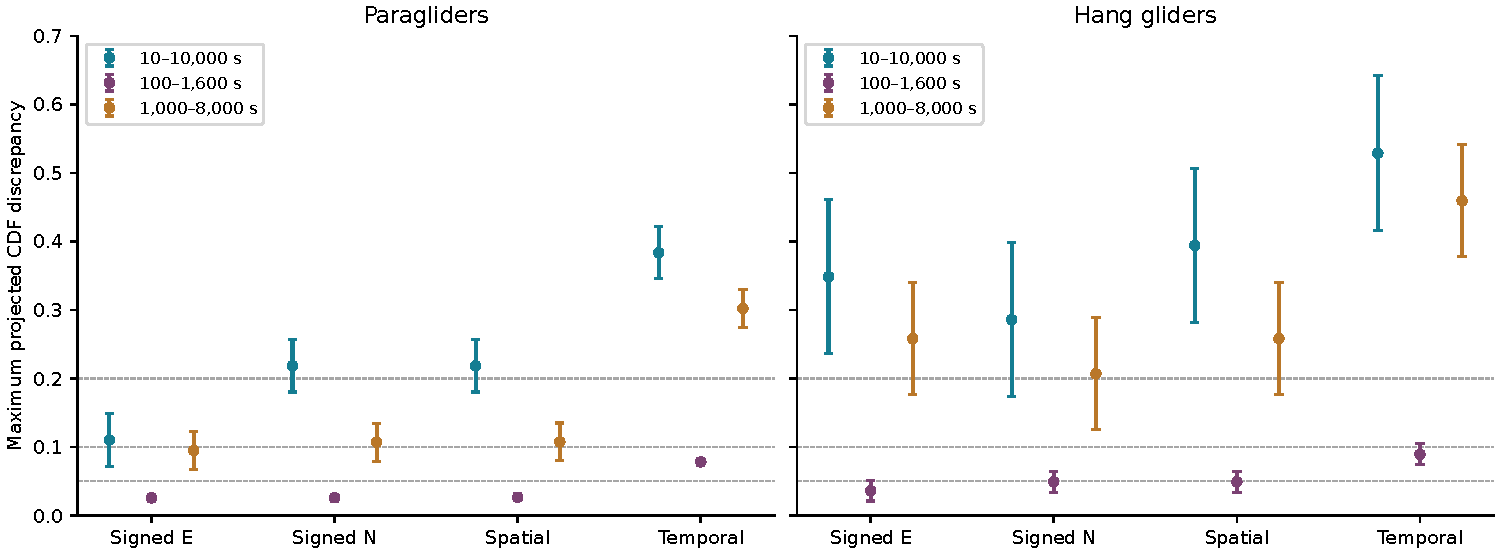
\includegraphics[width=\linewidth]{generated/ch3_temporal_scaling_distances}
 \caption{Held-out projected-CDF discrepancies and simultaneous 95\% bootstrap
 bounds. Dashed lines mark the declared tolerances. One common training exponent
 rescales all four coordinates. Each grid retains its own fixed population.}
 \label{fig:temporal-scaling-distances}
\end{figure}
\begin{table}[tb]
 \centering\small
 \caption{Maximum held-out projected-CDF discrepancy, with its simultaneous
 95\% upper bound in parentheses. A value of 0.05 means five percentage points
 of cumulative probability, not a 5\% relative error in displacement.}
 \label{tab:temporal-scaling-bounds}
 \begin{tabular}{llrrrr}
\toprule
 & Lag range (s) & Signed E & Signed N & Spatial & Temporal\\
\midrule
Para & 10--10000 & 0.110 (0.148) & 0.218 (0.257) & 0.218 (0.257) & 0.383 (0.422)\\
Para & 100--1600 & 0.026 (0.030) & 0.026 (0.031) & 0.026 (0.031) & 0.078 (0.083)\\
Para & 1000--8000 & 0.095 (0.122) & 0.107 (0.135) & 0.107 (0.135) & 0.302 (0.330)\\
Hang & 10--10000 & 0.349 (0.461) & 0.286 (0.399) & 0.394 (0.507) & 0.529 (0.642)\\
Hang & 100--1600 & 0.036 (0.051) & 0.049 (0.064) & 0.049 (0.064) & 0.089 (0.104)\\
Hang & 1000--8000 & 0.258 (0.340) & 0.207 (0.289) & 0.258 (0.340) & 0.459 (0.541)\\
\bottomrule
\end{tabular}

\end{table}

\paragraph{A supported intermediate-range approximation.}
On \SIrange{100}{1600}{\second}, the fitted exponents are 0.915 for
paragliders and 0.899 for hang gliders. For paragliders, the signed east,
north and spatial-projection discrepancies have upper bounds 0.0305, 0.0308
and 0.0313: all pass the declared 0.05 tolerance. Including temporal projections
raises the upper bound to 0.0829, still below 0.10. Hang-glider spatial
projections have upper bound 0.0640, below 0.10; their temporal discrepancy
is 0.0893 with upper bound 0.1043. The latter narrowly misses the declared
0.10 criterion and passes only the coarser 0.20 criterion.
Figures~\ref{fig:temporal-scaling-para} and~\ref{fig:temporal-scaling-hang}
show how the temporal difference exposes more separation than signed east
and north alone. The plotted lines interpolate the tested CDF thresholds;
they are not estimates of exact agreement between thresholds.

\begin{figure}[tb]
 \centering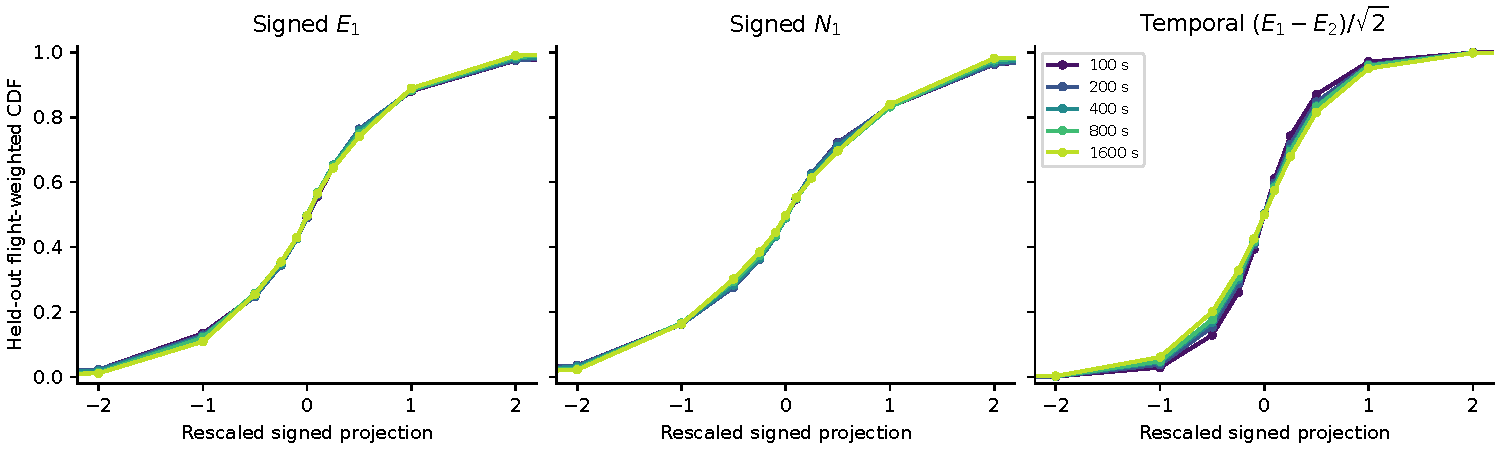
\includegraphics[width=\linewidth]{generated/ch3_temporal_scaling_para}
 \caption{Paraglider validation CDFs on the intermediate grid. The first two
 panels retain component signs; the last measures a projection involving both
 consecutive intervals. Each flight contributes the same total probability.}
 \label{fig:temporal-scaling-para}
\end{figure}
\begin{figure}[tb]
 \centering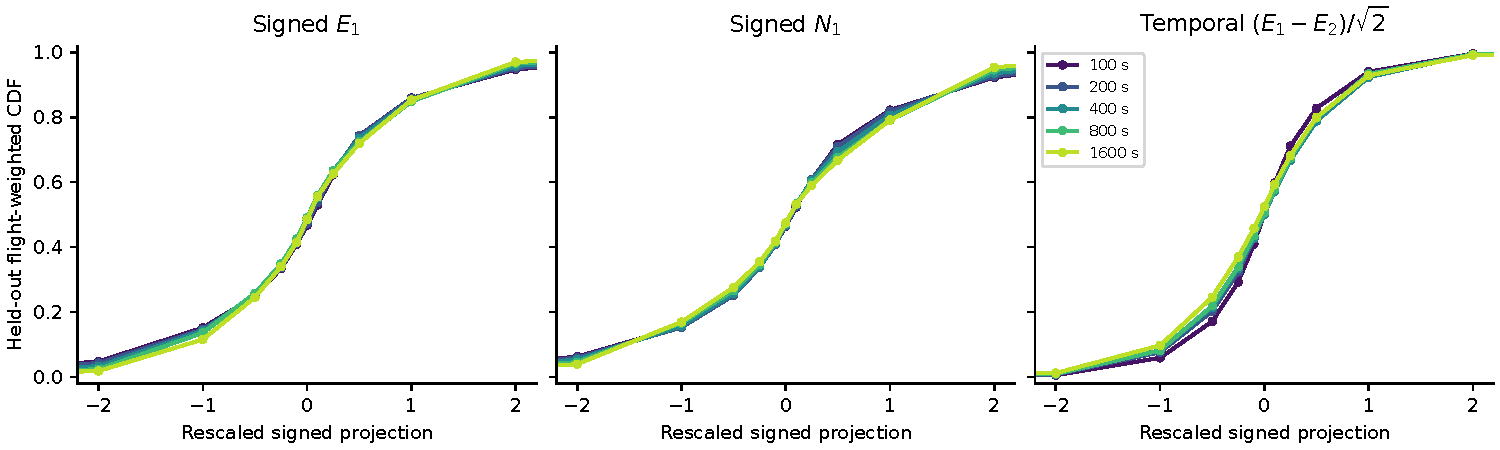
\includegraphics[width=\linewidth]{generated/ch3_temporal_scaling_hang}
 \caption{The same intermediate-grid signed and temporal comparison for hang
 gliders, using their independently fitted training exponent and length scale.}
 \label{fig:temporal-scaling-hang}
\end{figure}

The full and long grids give much larger temporal discrepancies: their lower
confidence bounds exceed 0.20 in both disciplines. Even on the intermediate
grid the discrepancies are resolved above zero, so exact invariance is not
supported. The positive conclusion is therefore \emph{approximate scalar
scaling of the signed spatial and tested two-interval laws over
\SIrange{100}{1600}{\second}}, strongest for paragliders. It is reasonable to
call this evidence for an approximate self-similar description on those scales,
provided its projection resolution, tolerances and population are stated.
It does not establish self-similarity for arbitrary observation times, increment
stationarity, or an intrinsic Hurst exponent. Small-scale manoeuvres and
longer-scale route constraints provide a plausible explanation for an
intermediate interval with better agreement; the present analysis does not
identify those mechanisms or disentangle them from cohort differences.
